\graphicspath{{./02-Projet/images/}}

\chapter{Introduction générale}
\label{chap:intro}
%\addcontentsline{toc}{section}{Introduction générale}

\section*{Contexte}
Cette thèse a été réalisée au sein du laboratoire 3SR de Grenoble dans lequel un axe de recherche a été développé afin d'optimiser la mise en forme de matériaux biosourcés à partir de poudre (ceux-ci se présentent généralement soit sous forme de poudre, soit sous forme de fibres).
\\Les matériaux biosourcés sont de plus en plus utilisés dans l'industrie de la fabrication dans le but de limiter l'utilisation de matériaux pétrosourcés, qui sont issus d'une ressource fragile aussi bien d'un point de vue écologique que économique. L'intérêt de mieux comprendre et de maîtriser ces matériaux est donc évident.
\\Une mise en forme par thermocompression a été privilégiée en raison de la possibilité qu'elle offre  de conserver les structures semi-cristallines natives des particules de poudre en optimisant les paramètres de mise en forme (température, temps de maintien, pression de confinement, ...). L'intérêt de conserver les structures natives est d'une part de minimiser la quantité d'énergie nécessaire à la transformation de ces matériaux, mais surtout de préserver les propriétés mécaniques natives souvent excellentes de ces matériaux. Il est par ailleurs très difficile, une fois la structure semi-cristalline native détériorée, de maîtriser artificiellement la recristallisation de ces matériaux pour obtenir des propriétés mécaniques similaires.
\begin{figure}\centering
	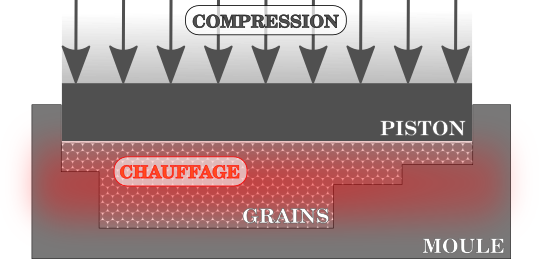
\includegraphics[width=0.5\textwidth]{compression.png}
	\caption{\label{fig:02-compression}Principe de mise en forme d'un matériau granulaire biosourcé par moulage}
\end{figure}
\\La figure~\ref{fig:02-compression} illustre la méthode de mise en forme choisie dans le laboratoire. Dans un premier temps, le matériau granulaire est introduit dans un moule qui définit la forme de la pièce finie. Une fois que le matériau granulaire, qui s'écoule tel un liquide, a pris la forme de l'empreinte du moule, un piston ayant une forme complémentaire au moule vient comprimer sous forte pression l'ensemble. La pression de confinement ainsi appliquée va permettre d'obtenir un matériau dense et, par conséquent, de meilleures caractéristiques mécaniques. Cette mise sous pression à froid suffit généralement à obtenir une pièce qui se tient mais dont les propriétés mécaniques restent faibles. C'est pour cette raison qu'il est nécessaire de chauffer le matériau, à une température modérée et éventuellement en présence d'une quantité limitée d'eau jouant le rôle de plastifiant, afin que les grains puissent créer des liaisons entre eux et ainsi améliorer les propriétés mécaniques de la pièce en sortie de moule. Si la température est trop grande, la température de fusion peut être atteinte et le matériau une fois refroidi ne possédera pas les mêmes propriétés mécaniques que celles des grains natifs. En revanche, pour des températures inférieures à celle de fusion, des liaisons interparticulaires peuvent être créées par des mécanismes de diffusion des macromolécules : il s'agit du frittage. Si la température est trop basse, l'énergie fournie au matériau ne suffit plus au frittage.
\\Le choix de la pression et de la température sont déterminants et le procédé de thermocompression permet de gérer l'énergie fournie au matériau pendant sa mise en forme assez facilement. Le procédé de thermocompression consiste à suivre les étapes mentionnées plus haut dans l'ordre : un piston vient comprimer la poudre à la pression voulue puis le moule est chauffé à la température souhaitée afin de diffuser la chaleur au sein de la poudre. Le pression et la température sont maintenues un certain temps. Une fois refroidie la pièce est éjectée. Ce procédé est assez lent (de l'ordre de l'heure) mais le contrôle des paramètres de mise en forme est facile et on observe une bonne reproductibilité. On peut également envisager un procédé de compression à froid suivi d'une phase de frittage qui permet d'augmenter les cadences de production : en effet la phase de compression est rapide (quelques secondes) et la phase de frittage plus longue (de l'ordre de l'heure). Ainsi il est possible de comprimer les pièces à la chaîne et de les placer ensuite en grand nombre dans un four de frittage afin de les traiter en même temps.

\section*{Un matériau biosourcé qui concurrence le plastique ?}
Le procédé de thermocompression a été mis en \oe{}uvre à l'échelle du laboratoire dans un précédent projet \textcolor{blue}{METTRE LES PUBLIS} sur des grains d'amidon de maïs. Afin d'optimiser les paramètres de mise en forme des deux procédés, de nombreux échantillons ont été produits avec différents paramètres. Les échantillons ont subi des tests de caractérisations mécaniques (flexion), physico-chimiques (DRX, densité) et microscopiques (MEB, AFM). La figure~\ref{fig:02-echantillons_amidon} présente un aperçu des échantillons ainsi réalisés.
\begin{figure}\centering
	\subfloat[]{
		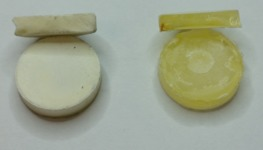
\includegraphics[height=110pt]{tablet.jpg}
		\label{subfig:02-tablet}
	}
	\subfloat[]{
		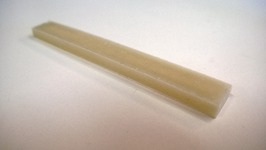
\includegraphics[height=110pt]{bar.jpg}
		\label{subfig:02-bar}
	}
	\caption{\label{fig:02-echantillons_amidon}\'Echantillons produits à partir des deux procédés de mise en forme : (a) pastilles créées par compression ultrasonore et (b) barre produite par thermocompression\textcolor{blue}{modifier la figure pour ne laisser que le (b) ??}}
\end{figure}
\\Il a été montré \textcolor{blue}{REF} qu'il est possible d'obtenir une pièce constituée d'un matériau dont la cristallinité native des grains est partiellement préservée. Cela permet au matériau de conserver les propriétés mécaniques et physico-chimiques des grains natifs. Les caractéristiques mécaniques dépendent également beaucoup de la densité apparente de la pièce produite.
\\Les pièces ayant les meilleures caractéristiques mécaniques et réalisées à partir des grains d'amidon de maïs ont vu leur porosité diminuer jusqu'à une valeur inférieure à $1\%$ pour les pièces dont les grains ont changé de phase durant le procédé (gélatinisation) et $10\%$ pour celles dont les grains ont conservé totalement ou partiellement leur structure.
\\D'un point de vue mécanique, les essais de flexion sur les éprouvettes issues de la thermocompression ont permis d'obtenir les caractéristiques présentées sur le tableau~\ref{tab:02-proprietes_thermocompression}.
\begin{table}\centering
	\begin{tabular}{>{\bfseries}r@{\hspace{10mm}}rl}
		\hline
		Comportement mécanique & \multicolumn{2}{c}{élastique - fragile} \\
		Module d'Young & $3~000$ & \SI{}{\mega\pascal} \\
		Contrainte en flexion & $10$ & \SI{}{\mega\pascal} \\
		Déformation à rupture & $0.4$ & \SI{}{\%} \\
		Porosité & $3$ & \% \\
		Pression de confinement & de $25$ à $100$ & \SI{}{\mega\pascal} \\
		Cristallinité & \multicolumn{2}{c}{bien préservée} \\
		\hline
	\end{tabular}
	\caption{\label{tab:02-proprietes_thermocompression}Propriétés atteintes par les échantillons moulés par thermocompression}
\end{table}
\\On s'aperçoit, en regardant le tableau~\ref{tab:02-proprietes_thermocompression} qu'un tel matériau possède d'assez bonnes caractéristiques mécaniques pour remplacer certains thermoplastiques largement utilisés dans l'industrie de la fabrication tels que les polyéthylènes de faibles et moyennes densités. En ajoutant même des fibres naturelles, il est possible de produire un composite biosourcé à $100\%$ et dont les propriétés mécaniques dépassent celles du polycarbonate ou du PVC \citep{wypych_handbook_2016}.
\\Cependant, un certain nombre de défauts, notamments de microfissures, ont été observés sur les échantillons, montrant ainsi une perspective d'amélioration significative des propriétés mécaniques présentées sur le tableau~\ref{tab:02-proprietes_thermocompression}. Il est probable que les fissures soient dues au retrait thermique lié à un refroidissement mal maîtrisé. Pour améliorer ces propriétés, l'une des perspectives est d'améliorer le procédé jusqu'alors utiliser en maîtrisant le refroidissement tout en maintenant les contraintes mécaniques. Une autre perspective est d'investiguer la compression à froid, de manière à chauffer l'échantillon libre de contraintes. Ainsi les contraintes de traction qui peuvent apparaître au démoulage ne viennent pas rompre les interfaces intergranulaires encore fragiles. Dans ce cas, la contrainte de compression peut être augmentée afin de diminuer au maximum la porosité sans l'appui de la température. On se rapproche alors très fortement du procédé classique de compression à froid - frittage mentionné plus haut.

Dans tous les cas, il est apparu lors du projet une envie forte de comprendre l'évolution de la microstructure de ces matériaux et les mécanismes d'établissement des surfaces de contact intergranulaires lors de la compression. Le présent projet de thèse a alors été imaginé, dont l'objectif à long terme est de comprendre par la modélisation à l'échelle des particules, les mécanismes de fissuration pouvant mener aux défauts mentionnés ci-dessus. L'étude exposée dans ce mémoire est le premier pas dans cette direction: son objectif est d'établir des outils de modélisation couplés aux techniques de microtomographie aux rayons X et d'analyse d'image 3D bien maîtrisées au laboratoire 3SR. On comprendra que les outils développés ont un champ d'applications potentielles bien plus large que le projet décrit ci-dessous.

\section*{Un matériau modèle pour l'étude}
Bien que le projet scientifique à l'origine des travaux réalisés dans cette thèse ait pour objectif de comprendre le comportement de la poudre d'amidon lors d'une phase de mise en forme, le choix d'utiliser un matériau modèle qui ne soit pas de l'amidon a été fait. Le polystyrène a été choisi comme matériau modèle dans les travaux présentés dans cet ouvrage. Bien que issu de l'industrie pétrochimique, ce matériau polymère a été choisi pour différentes raisons : ses propriétés physiques et chimiques ont été assez largement étudiées, et donc bien connues, il est très disponible car beaucoup utilisé dans le secteur industriel et il peut également être livré sous forme de poudre. Les raisons principales de ce choix résident dans les faits que, d'une part le comportement mécanique du polystyrène est comparable à celui de l'amidon (ce sont des polymères dans les deux cas, ils ont un comportement viscoélastique et peuvent être fragiles ou ductiles suivant les conditions) et d'autre part, le polystyrène offre la possibilité de travailler sur des grains dont la taille est supérieure (plusieurs centaines de microns comparé à une dizaine de microns pour l'amidon de maïs), ce qui permet l'analyse par imagerie 3D avec le tomgraphe du laboratoire dont la résolution est limitée à quelques microns. En plus de cela, la forme complexe des grains obtenus par cryofracture permet d'envisager l'analyse de milieux constitués de grains irréguliers.

\section*{Objectif des travaux de thèse}
Les travaux de thèse qui sont présentés dans cet ouvrage ont pour objectif de développer un méthode qui permette de mieux comprendre les relations entre la microstructure d'un milieu granulaire et ses propriétés mécaniques. Une des applications de ces travaux pourrait être l'étude du comportement mécanique d'un matériau granulaire biosourcé soumis à des efforts de compression. Dans tous les cas, il s'agit d'un matériau granulaire constitués de grains sui subissent une déformation importante lors de la mise en forme, ce qui le distingue des matériaux granulaires rencontrés en mécanique des sols et qui ont fait l'objet de très nombreuses études. Il a été vu dans les paragraphes précédents que la mise en forme d'un tel matériau nécessite deux étapes : une compression et un frittage. Les résultats présentés ici serviraient alors à l'analyse de cette première étape.
\\Il est possible de distinguer deux approches complémentaires l'une de l'autre dans les travaux qui suivent. En effet, une approche expérimentale permet d'étudier le comportement mécanique et la microstructure d'un milieu granulaire, dans sa globalité, soumis à un chargement triaxial ; mais aussi, une approche numérique permet, quant à elle, d'extraire la microstructure du milieu granulaire et de déterminer les champs de densité et la cinématique locale afin de procéder à des simulations numériques pouvant être directement comparées à l'expérimentation.
\begin{itemize}
	\item \textbf{Approche expérimentale} : des essais de compression ont été menés sur le matériau granulaire. Il s'agit d'essais de compression triaxiale de révolution qui sont présentés en détail dans le paragraphe \ref{para03:triax}. Les courbes de contraintes et de déformations déduites de cet essai permettent d'interpréter le comportement mécanique de l'ensemble des grains lorsque le matériau est confiné sous une certaine pression et soumis à une pression supplémentaire dans une direction. Lorsque les essais sont réalisés à l'intérieur même d'un tomographe de laboratoire (plus de détails sur la tomographie à rayons X au paragraphe \ref{para03:tomo}), il est alors possible d'observer la microstructure de l'ensemble de l'échantillon durant le test. Cette microstructure nous informe sur la densité du milieu ainsi que sur la cinématique des grains en étudiant les différents états de compression. Les champs de densité, déplacements et déformations sont alors connus localement et globalement grâce à la tomographie tandis que les mesures des capteurs de forces durant l'essai permettent de connaître la réponse globale du système aux conditions imposées.
	\item \textbf{Approche numérique} : des essais de compression ont été menés sur des échantillons numériques afin de simuler l'essai expérimental. Pour cela, la méthode de simulation choisie est celle des éléments finis multi-particules (voir le paragraphe \ref{para03:MPFEM}). L'utilisation des éléments finis a l'avantage de reproduire fidèlement la géométrie des grains, mais aussi de tenir compte des déformations des grains. Grâce à la tomographie réalisée durant les essais de compression, les simulations sont basées sur les expérimentations :
	\begin{itemize}
		\item Les échantillons numériques sont produits à partir des échantillons réels. A chaque étape de compression, les images de tomographie permettent d'obtenir la géométrie entière de l'ensemble des grains constituant l'échantillon. A l'aide d'un algorithme de traitement d'image sur l'état initial de la compression (avant la mise en confinement), il est possible d'individualiser les grains afin d'avoir une "version numérisée" de chacun d'entre eux et d'enregistrer l'agencement réel des grains. Ainsi, une bibliothèque de grains est créée et un assemblage cohérent des grains entre eux est réalisé. \emph{Les grains numérisés sont les images presque parfaites des grains réels}.
		\item Les images de tomographie permettent de réaliser une corrélation d'images volumiques entre chaque étape de compression. Une interpolation linéaire de la corrélation des volumes rend possible le fait de connaître l'emplacement de chaque grain et donc leur déplacement à chaque étape. Les déplacements observés par la corrélation d'images vont être directement utilisés dans la simulation numérique comme conditions aux limites. Aux hypothèses près, \emph{les déplacements des grains numérisés aux frontières sont ceux des grains réels}.
	\end{itemize}
	Avec l'approche numérique il est possible de simuler un même test sur un matériau dont les propriétés sont modifiées afin de mieux comprendre l'effet de chacune de ses propriétés. L'inverse est également possible : il est possible de modifier des conditions de test avec un matériau identique pour mieux comprendre l'effet des conditions expérimentales. On voit ici tout l'intérêt du travail numérique.
\end{itemize}
Ces deux approches, expérimentale et numérique, sont complémentaires pour l'étude du comportement mécanique de la poudre sous compression. Les simulations numériques étant fortement basées sur les expérimentations, il est alors très intéressant de mener une étude de comparaison entre les deux approches. Cela permet de mieux cibler les phénomènes en jeu lors de la compression.
\paragraph{}En plus des résultats observés lors des travaux expérimentaux et numériques, cette thèse présente une nouvelle méthode de modélisation d'un matériau granulaire sous chargement mécanique. Cette méthode est présentée graphiquement sur la figure~\ref{fig:02-method} et consiste à utiliser l'ensemble d'une expérimentation dans une simulation numérique.
\begin{figure}\centering
	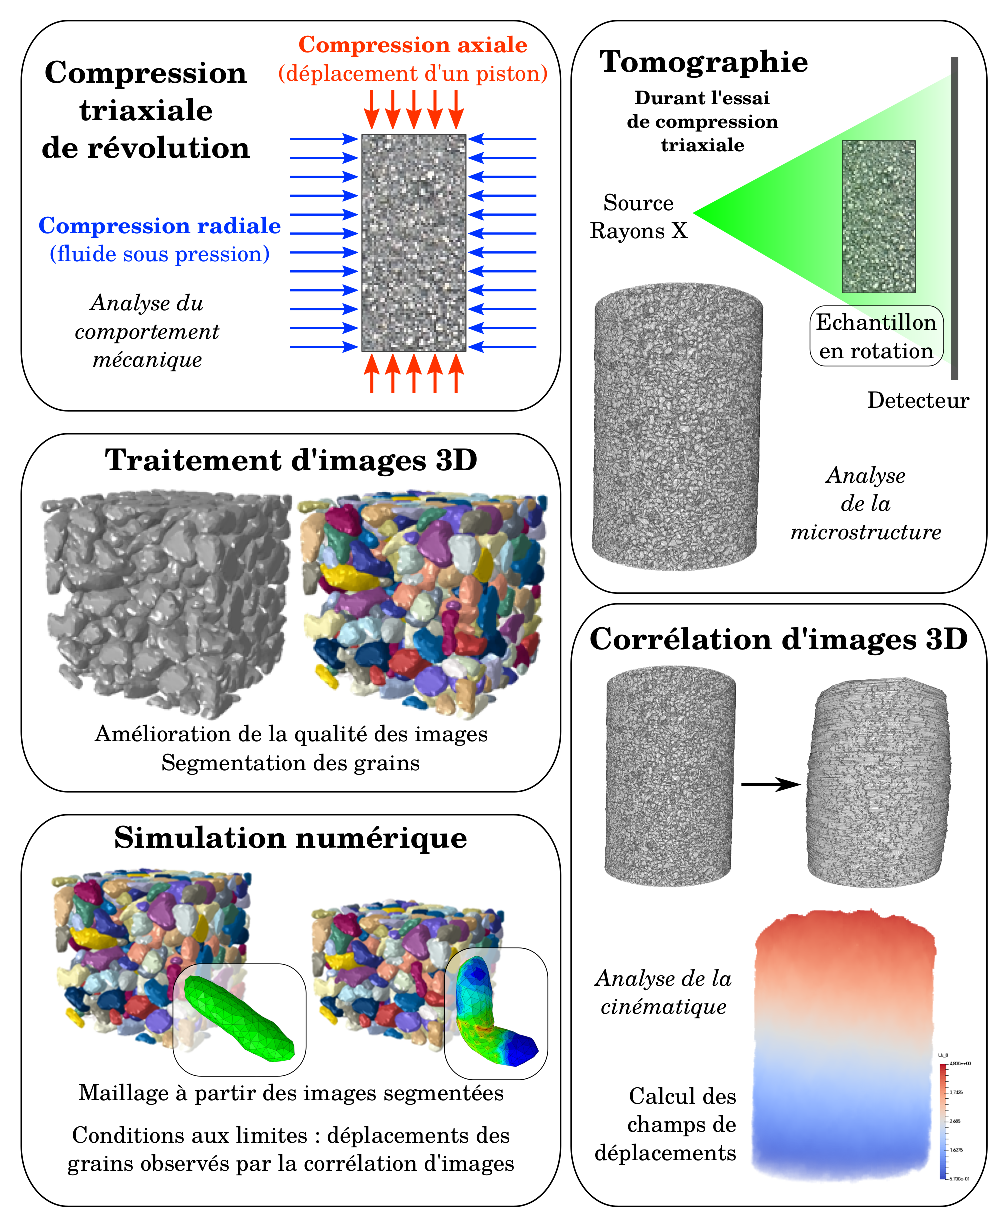
\includegraphics[width=0.95\textwidth]{method.eps}
	\caption{\label{fig:02-method}Les différentes étapes des travaux réalisés}
\end{figure}